 \hypertarget{a00380_termsanddefs_objects}{}\section{Objects}\label{a00380_termsanddefs_objects}

\begin{DoxyDescription}
\item[Object ]Interesting kind of part of the system, such as a Core, a L2\+Cache, a N\+U\+MA memory node, etc. The different types detected by hwloc are detailed in the \hyperlink{a00184_gacd37bb612667dc437d66bfb175a8dc55}{hwloc\+\_\+obj\+\_\+type\+\_\+t} enumeration.

There are four kinds of Objects\+: Memory (N\+U\+MA nodes and Memory-\/side caches), I/O (Bridges, P\+CI and OS devices), Misc, and Normal (everything else, including Machine, Package, Die, Core, PU, C\+PU Caches, etc.). Normal and Memory objects have (non-\/\+N\+U\+LL) C\+PU sets and nodesets, while I/O and Misc don\textquotesingle{}t.

Objects are topologically sorted by locality (C\+PU and node sets) into a tree (see \hyperlink{a00380_termsanddefs_tree}{Hierarchy, Tree and Levels}). 


\item[Processing Unit (PU) ]The smallest processing element that can be represented by a hwloc object. It may be a single-\/core processor, a core of a multicore processor, or a single thread in a S\+MT processor (also sometimes called \char`\"{}\+Logical processor\char`\"{}, not to be confused with \char`\"{}\+Logical index of a processor\char`\"{}). hwloc\textquotesingle{}s PU acronym stands for Processing Unit. 


\item[Package ]A processor Package is the physical package that usually gets inserted into a socket on the motherboard. It is also often called a physical processor or a C\+PU even if these names bring confusion with respect to cores and processing units. A processor package usually contains multiple cores (and may also be composed of multiple dies). hwloc Package objects were called Sockets up to hwloc 1.\+10. 


\item[N\+U\+MA Node ]An object that contains memory that is directly and byte-\/accessible to the host processors. It is usually close to some cores as specified by its C\+PU set. Hence it is attached as a memory child of the object that groups those cores together, for instance a Package objects with 4 Core children (see \hyperlink{a00380_termsanddefs_tree}{Hierarchy, Tree and Levels}). 


\item[Memory-\/side Cache ]A cache in front of a specific memory region (e.\+g. a range of physical addresses). It caches all accesses to that region without caring about which core issued the request. This is the opposite of usual C\+PU caches where only accesses from the local cores are cached, without caring about the target memory.

In hwloc, memory-\/side caches are memory objects placed between their local C\+PU objects (parent) and the target N\+U\+MA node memory (child).  
\end{DoxyDescription}

 \hypertarget{a00380_termsanddefs_indexes}{}\section{Indexes and Sets}\label{a00380_termsanddefs_indexes}

\begin{DoxyDescription}
\item[OS or physical index ]The index that the operating system (OS) uses to identify the object. This may be completely arbitrary, non-\/unique, non-\/contiguous, not representative of logical proximity, and may depend on the B\+I\+OS configuration. That is why hwloc almost never uses them, only in the default lstopo output ({\ttfamily P\#x}) and cpuset masks. See also \hyperlink{a00394_faq_indexes}{Should I use logical or physical/\+OS indexes? and how?}.


\item[Logical index ]Index to uniquely identify objects of the same type and depth, automatically computed by hwloc according to the topology. It expresses logical proximity in a generic way, i.\+e. objects which have adjacent logical indexes are adjacent in the topology. That is why hwloc almost always uses it in its A\+PI, since it expresses logical proximity. They can be shown (as {\ttfamily L\#x}) by {\ttfamily lstopo} thanks to the {\ttfamily -\/l} option. This index is always linear and in the range \mbox{[}0, num\+\_\+objs\+\_\+same\+\_\+type\+\_\+same\+\_\+level-\/1\mbox{]}. Think of it as ``cousin rank.\textquotesingle{}\textquotesingle{} The ordering is based on topology first, and then on OS C\+PU numbers, so it is stable across everything except firmware C\+PU renumbering. \char`\"{}\+Logical index\char`\"{} should not be confused with \char`\"{}\+Logical processor\char`\"{}. A \char`\"{}\+Logical
  processor\char`\"{} (which in hwloc we rather call \char`\"{}processing unit\char`\"{} to avoid the confusion) has both a physical index (as chosen arbitrarily by B\+I\+O\+S/\+OS) and a logical index (as computed according to logical proximity by hwloc). See also \hyperlink{a00394_faq_indexes}{Should I use logical or physical/\+OS indexes? and how?}.


\item[C\+PU set ]The set of processing units (PU) logically included in an object (if it makes sense). They are always expressed using physical processor numbers (as announced by the OS). They are implemented as the \hyperlink{a00205_gaa3c2bf4c776d603dcebbb61b0c923d84}{hwloc\+\_\+bitmap\+\_\+t} opaque structure. hwloc C\+PU sets are just masks, they do {\itshape not} have any relation with an operating system actual binding notion like Linux\textquotesingle{} cpusets. I/O and Misc objects do not have C\+PU sets while all Normal and Memory objects have non-\/\+N\+U\+LL C\+PU sets.


\item[Node set ]The set of N\+U\+MA memory nodes logically included in an object (if it makes sense). They are always expressed using physical node numbers (as announced by the OS). They are implemented with the \hyperlink{a00205_gaa3c2bf4c776d603dcebbb61b0c923d84}{hwloc\+\_\+bitmap\+\_\+t} opaque structure. as bitmaps. I/O and Misc objects do not have Node sets while all Normal and Memory objects have non-\/\+N\+U\+LL nodesets.


\item[Bitmap ]A possibly-\/infinite set of bits used for describing sets of objects such as C\+P\+Us (C\+PU sets) or memory nodes (Node sets). They are implemented with the \hyperlink{a00205_gaa3c2bf4c776d603dcebbb61b0c923d84}{hwloc\+\_\+bitmap\+\_\+t} opaque structure. 


\end{DoxyDescription}

 \hypertarget{a00380_termsanddefs_tree}{}\section{Hierarchy, Tree and Levels}\label{a00380_termsanddefs_tree}

\begin{DoxyDescription}
\item[Parent object ]The object logically containing the current object, for example because its C\+PU set includes the C\+PU set of the current object. All objects have a non-\/\+N\+U\+LL parent, except the root of the topology (Machine object). 


\item[Ancestor object ]The parent object, or its own parent, and so on.


\item[Children object(s) ]The object (or objects) contained in the current object because their C\+PU set is included in the C\+PU set of the current object. Each object may also contain separated lists for Memory, I/O and Misc object children. 


\item[Arity ]The number of normal children of an object. There are also specific arities for Memory, I/O and Misc children. 


\item[Sibling objects ]Objects in the same children list, which all of them are normal children of the same parent, or all of them are Memory children of the same parent, or I/O children, or Misc. They usually have the same type (and hence are cousins, as well). But they may not if the topology is asymmetric. 


\item[Sibling rank ]Index to uniquely identify objects which have the same parent, and is always in the range \mbox{[}0, arity-\/1\mbox{]} (respectively memory\+\_\+arity, io\+\_\+arity or misc\+\_\+arity for Memory, I/O and Misc children of a parent).


\item[Cousin objects ]Objects of the same type (and depth) as the current object, even if they do not have the same parent.


\item[Level ]Set of objects of the same type and depth. All these objects are cousins.

Memory, I/O and Misc objects also have their own specific levels and (virtual) depth. 


\item[Depth ]Nesting level in the object tree, starting from the root object. If the topology is symmetric, the depth of a child is equal to the parent depth plus one, and an object depth is also equal to the number of parent/child links between the root object and the given object. If the topology is asymmetric, the difference between some parent and child depths may be larger than one when some intermediate levels (for instance groups) are missing in only some parts of the machine.

The depth of the Machine object is always 0 since it is always the root of the topology. The depth of PU objects is equal to the number of levels in the topology minus one.

Memory, I/O and Misc objects also have their own specific levels and depth. 


\end{DoxyDescription}

The following diagram can help to understand the vocabulary of the relationships by showing the example of a machine with two dual core packages (with no hardware threads); thus, a topology with 5 levels. Each box with rounded corner corresponds to one \hyperlink{a00185_ga79b8ab56877ef99ac59b833203391c7d}{hwloc\+\_\+obj\+\_\+t}, containing the values of the different integer fields (depth, logical\+\_\+index, etc.), and arrows show to which other \hyperlink{a00185_ga79b8ab56877ef99ac59b833203391c7d}{hwloc\+\_\+obj\+\_\+t} pointers point to (first\+\_\+child, parent, etc.).

The topology always starts with a Machine object as root (depth 0) and ends with PU objects at the bottom (depth 4 here).

Objects of the same level (cousins) are listed in red boxes and linked with red arrows. Children of the same parent (siblings) are linked with blue arrows.

The L2 cache of the last core is intentionally missing to show how asymmetric topologies are handled. See \hyperlink{a00394_faq_asymmetric}{What happens if my topology is asymmetric?} for more information about such strange topologies.

 
\begin{DoxyImageNoCaption}
  \mbox{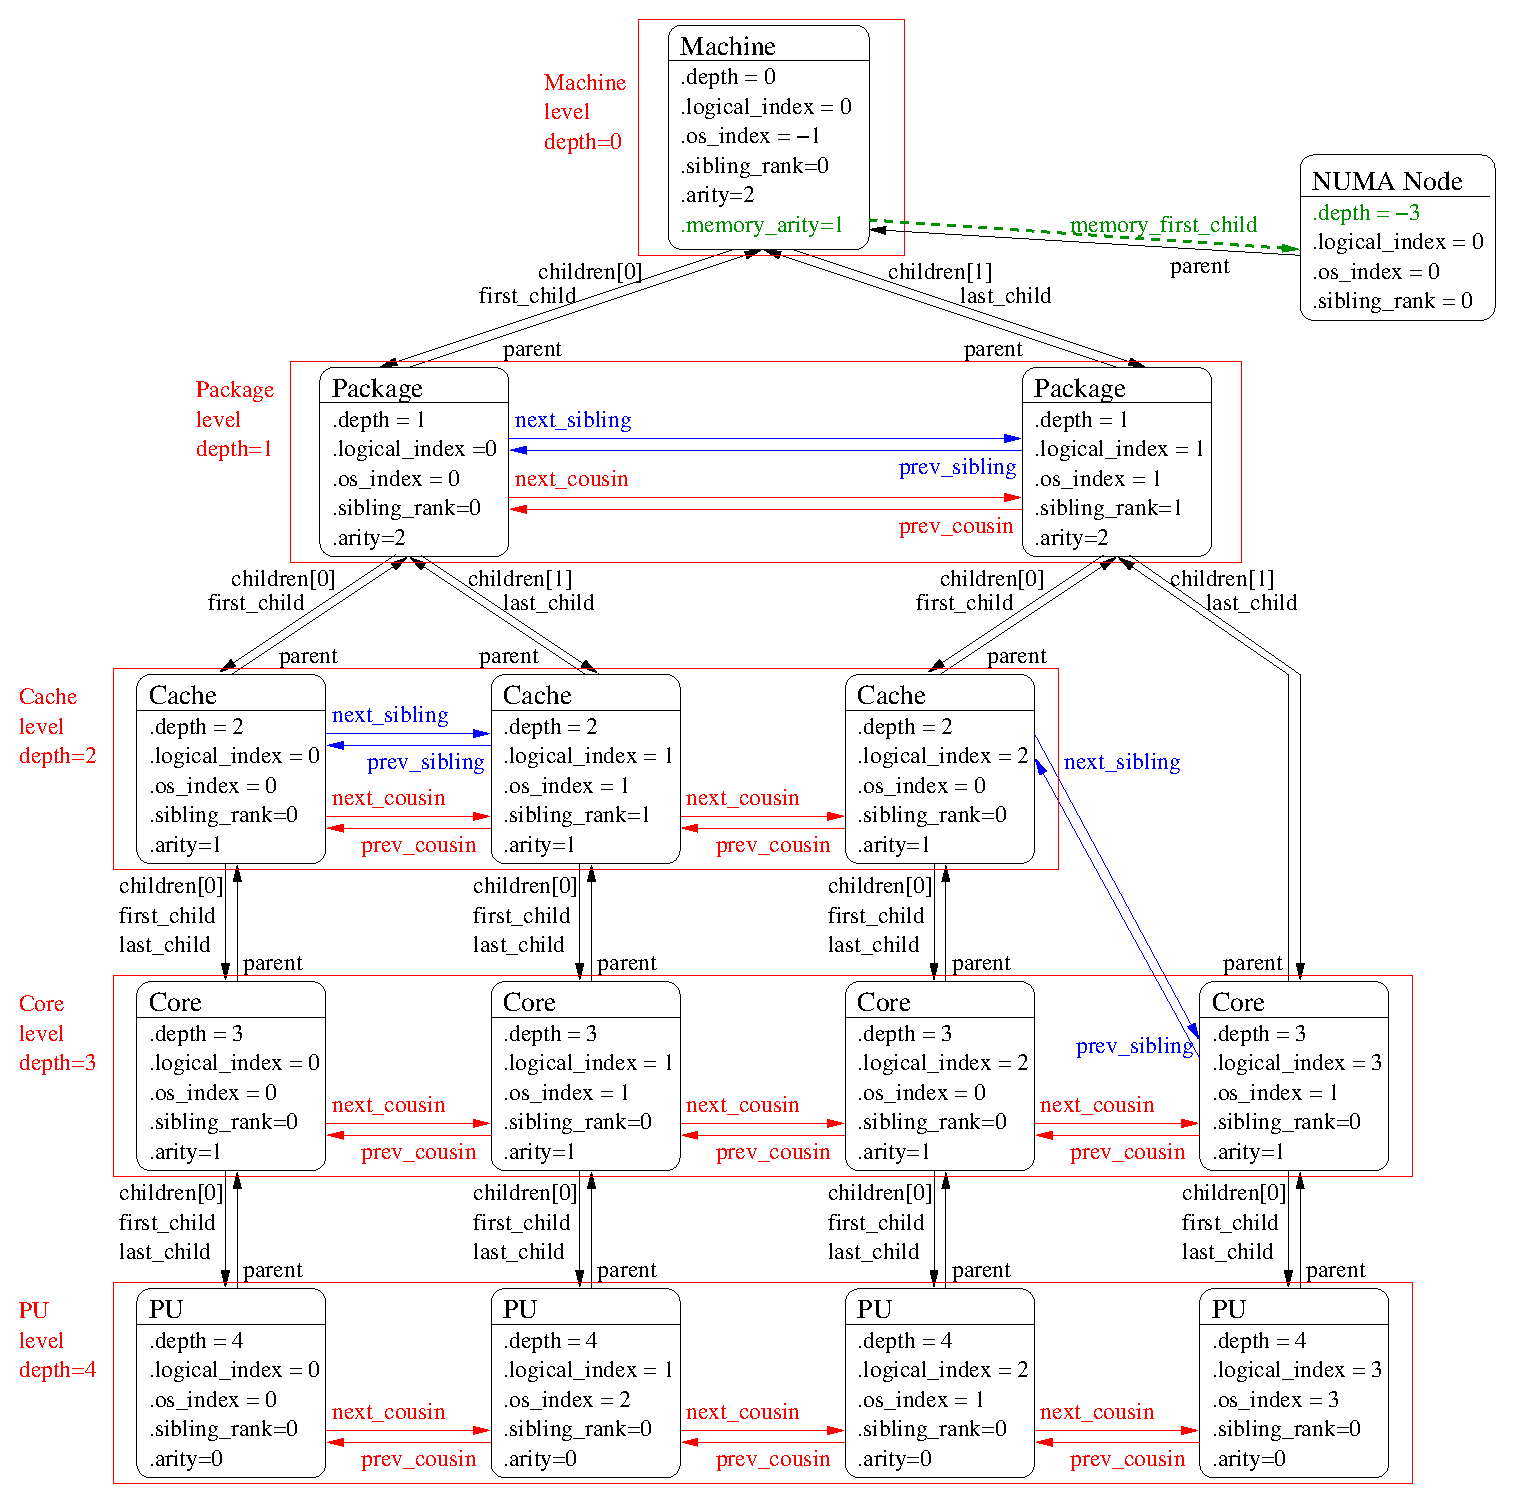
\includegraphics[width=\textwidth]{diagram}}
\end{DoxyImageNoCaption}


It should be noted that for PU objects, the logical index -- as computed linearly by hwloc -- is not the same as the OS index.

The N\+U\+MA node is on the side because it is not part of the main tree but rather attached to the object that corresponds to its locality (the entire machine here, hence the root object). It is attached as a {\itshape Memory} child (in green) and has a virtual depth (negative). It could also have siblings if there were multiple local N\+U\+MA nodes, or cousins if other N\+U\+MA nodes were attached somewhere else in the machine.

I/O or Misc objects could be attached in a similar manner. 